Qui di seguito è riportato uno schema logico del database mediante modello Relazionale.
\begin{figure}[htp]
\centering
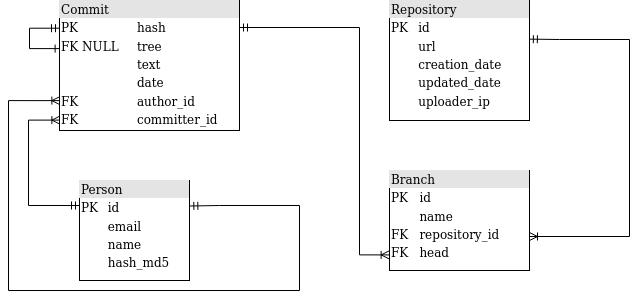
\includegraphics[scale=0.70]{data/relation.png}
\caption{Modello relazionale}
\label{}
\end{figure}

Come si può ben vedere sono state fatte delle modifiche:
\begin{itemize}
\item Repository: aggiunte le date di creazione e modifica;
\item Branch: ha un suo id come PK, in modo da accedervi più facilmente tramite backend. Questo perché i branch permettono anche lo slash nel nome, cosa che andrebbe a creare errore se passato nell'endpoint;
\item Commit: ha un campo \verb|tree| che si riferisce al parent: può ovviamente essere null. Dato che il commit può essere scritto da massimo 2 persone, ho preferito aggiungere i campi \verb|author_id| e \verb|commiter_id|;
\item Person: ha un campo \verb|hash_md5| che calcola l'MD5\footnote{https://en.wikipedia.org/wiki/MD5} dell'email una volta sola: usato per il gravatar;
\end{itemize}
